\documentclass[a4paper,12pt]{article}
\usepackage[utf8]{inputenc}
\usepackage{amsmath, amssymb}
\usepackage{graphicx}
\usepackage{geometry}
\geometry{margin=1in}


\title{Independent Component Analysis for Signal Separation}
\author{Hamza LOUKILI}
\date{\today}

\begin{document}

% Page de garde avec image
\begin{titlepage}
    \centering
    % Image de fond (ajuster le chemin du fichier)


     
    
    % Texte sur la page de garde
    \Huge
    \textbf{Independent Component Analysis for Signal Separation} \\[1cm]
    \Large
    Hamza LOUKILI \\
    \large
    \today \\
    \vspace{2cm}
    
    
\includegraphics[width=0.3\textwidth]{figures/cocktail_party.jpeg}
\end{titlepage}


\tableofcontents

\newpage
\section{Introduction}

In our modern world, signals are ubiquitous, emanating from a multitude of independent sources and often becoming entangled in complex mixtures. Examples include the overlapping voices in a crowded room, the combined readings from multiple sensors, or the superimposed signals in biomedical recordings. The challenge of isolating these original, underlying source signals from their observed mixtures is critical for meaningful analysis and interpretation. This process, known as \emph{signal separation}, seeks to recover the individual source signals without prior knowledge of their characteristics or the mixing process.

Among the numerous techniques developed to address this challenge, Independent Component Analysis (ICA) stands out as a powerful and versatile statistical method. Unlike traditional approaches, which often rely on assumptions about the spectral or temporal properties of the signals, ICA exploits a fundamental statistical property: the independence of the source signals. This enables ICA to perform \emph{blind source separation}, meaning it can effectively disentangle the sources even when little to no information about the mixing process or the sources themselves is available.

The core principle of ICA is to find a linear transformation of the observed mixed signals that renders the resulting components as statistically independent as possible. This is achieved by leveraging higher-order statistics of the data, going beyond the second-order statistics (such as correlation) used in methods like Principal Component Analysis (PCA). By doing so, ICA can uncover the latent structure of the data, making it particularly well-suited for applications where the sources are mixed in unknown ways.

This report provides a comprehensive exploration of the principles and applications of ICA for signal separation. The following sections are structured as follows: first, we establish a theoretical foundation for ICA, detailing its mathematical framework and key assumptions. Then, we examine practical applications of ICA across various domains, demonstrating its effectiveness in addressing real-world signal separation challenges.

\newpage

\section{Theoretical Foundation of ICA}

At its core, ICA addresses the problem of recovering a set of unobserved, statistically independent source signals, denoted as 

\[
\mathbf{s}(t) = [s_1(t), s_2(t), \dots, s_n(t)]^T,
\]

from a set of observed mixtures,

\[
\mathbf{x}(t) = [x_1(t), x_2(t), \dots, x_m(t)]^T.
\]

The fundamental assumption in the basic linear instantaneous ICA model is that the observed signals are linear combinations of the source signals. This relationship can be expressed mathematically as:

\begin{equation}
\mathbf{x}(t) = \mathbf{A} \mathbf{s}(t),
\end{equation}

where:
\begin{itemize}
    \item \(\mathbf{x}(t) \in \mathbb{R}^m\) is the \(m\)-dimensional vector of observed mixtures at time \(t\),
    \item \(\mathbf{s}(t) \in \mathbb{R}^n\) is the \(n\)-dimensional vector of unknown source signals at time \(t\),
    \item \(\mathbf{A} \in \mathbb{R}^{m \times n}\) is the unknown mixing matrix, with each element \(a_{ij}\) representing the contribution of the \(j\)-th source signal to the \(i\)-th observed mixture.
\end{itemize}

\begin{figure}
    \centering
    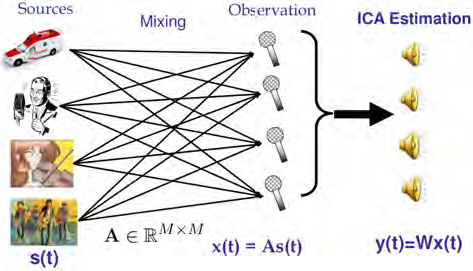
\includegraphics[width=0.5\linewidth]{figures/ica_separation.png}
    \caption{Illustration}
    \label{image_sep}
\end{figure}

For simplicity, we often assume that the number of observed mixtures equals the number of source signals (\(m = n\)), and that the mixing matrix \(\mathbf{A}\) is invertible. Under these conditions, the goal of ICA is to estimate an unmixing matrix \(\mathbf{W}\) such that:

\begin{equation}
\mathbf{y}(t) = \mathbf{W} \mathbf{x}(t) = \mathbf{W} \mathbf{A} \mathbf{s}(t) \approx \mathbf{s}(t),
\end{equation}

where \(\mathbf{y}(t) \in \mathbb{R}^n\) is the \(n\)-dimensional vector of estimated source signals. Ideally, \(\mathbf{W}\) is the inverse of \(\mathbf{A}\), up to permutation and scaling ambiguities, which will be discussed later.

\subsection{Assumption of Statistical Independence}

The cornerstone of ICA is the assumption of \emph{statistical independence} among the source signals \(s_i(t)\). This implies that the joint probability distribution of the source signals can be factored into the product of their marginal probability distributions:

\begin{equation}
P(s_1, s_2, \dots, s_n) = P(s_1) P(s_2) \cdots P(s_n).
\end{equation}

This assumption is pivotal, as it enables ICA to distinguish between independent sources that may appear correlated in the observed mixtures.

\subsection{Assumption of Non-Gaussianity}

Another critical assumption in many ICA algorithms is that the source signals are \emph{non-Gaussian}. This is essential because, if the sources were Gaussian, the mixing process would result in mixtures that are also Gaussian, and it would be impossible to uniquely determine the mixing matrix based solely on the observed data, due to the rotational symmetry of Gaussian distributions. A key insight in ICA is rooted in the Central Limit Theorem, which states that linear mixtures of independent random variables tend to be "more Gaussian" than the original variables. Consequently, to recover the independent components, ICA algorithms seek linear transformations of the observed mixtures that maximize their non-Gaussianity.

\subsection{Mathematical Criteria for ICA}

Several mathematical principles and measures are employed in ICA algorithms to achieve this separation, including:

\subsubsection{Maximization of Non-Gaussianity}

Measures such as kurtosis (the fourth-order cumulant) and negentropy (a measure of distance from Gaussianity based on information theory) are often used as objective functions to be maximized. For instance, kurtosis is defined as:

\begin{equation}
\text{kurt}(y) = E[y^4] - 3(E[y^2])^2,
\end{equation}

where positive kurtosis indicates a "spikier" distribution than Gaussian, and negative kurtosis indicates a "flatter" distribution.

\subsubsection{Minimization of Mutual Information}

Mutual information quantifies the statistical dependence between random variables. ICA aims to find a transformation that minimizes the mutual information between the estimated source signals, thereby ensuring their independence. Mutual information \(I(\mathbf{y})\) between the components of \(\mathbf{y}\) is defined as:

\begin{equation}
I(\mathbf{y}) = \sum_{i=1}^n H(y_i) - H(\mathbf{y}),
\end{equation}

where \(H(y_i)\) is the entropy of the \(i\)-th component, and \(H(\mathbf{y})\) is the joint entropy of \(\mathbf{y}\).

\subsubsection{Maximum Likelihood Estimation}

Under certain assumptions about the probability distributions of the source signals (e.g., Laplacian or logistic distributions), the unmixing matrix can be estimated by maximizing the likelihood of the observed data. The likelihood function is given by:

\begin{equation}
L(\mathbf{W}) = \prod_{t=1}^T P(\mathbf{x}(t) \mid \mathbf{W}) = \prod_{t=1}^T |\det(\mathbf{W})| \prod_{i=1}^n P_s(y_i(t)),
\end{equation}

where \(P_s(\cdot)\) is the probability density function of the source signals.

\newpage
\section{Application of ICA}

Independent Component Analysis (ICA) is a powerful technique for separating mixed signals and recovering independent sources. It is particularly useful when the original sources are unknown, but only their mixtures are observed. This capability has significant practical applications in various fields where isolating signals from overlapping sources is crucial.

\subsection{Applications in Various Fields}

ICA is widely employed across multiple disciplines, including:

\begin{itemize}
    \item Audio signal processing: ICA can separate mixed audio signals, such as voices recorded in noisy environments, making it valuable in telecommunications, speech recognition, and audio enhancement.
    
    \item Neuroscience and EEG analysis: ICA helps isolate brain signals from external artifacts in electroencephalogram (EEG) recordings, aiding neurological studies and medical diagnostics.
    
    \item Image processing: ICA is used in computer vision for tasks such as image segmentation and feature extraction, helping to uncover underlying structures in complex images.
    
    \item Financial data analysis: ICA can extract independent factors influencing stock market trends and other economic signals, facilitating better financial modeling and risk assessment.
    
    \item Biomedical signal processing: ICA improves the quality of biomedical data, such as electrocardiograms (ECG), by separating relevant signals from noise and artifacts, enhancing medical diagnoses.
\end{itemize}

\subsection{Our Application: Sound Separation Using ICA}

In this study, we applied ICA to separate artificially mixed audio signals, demonstrating its effectiveness in practical scenarios.

\subsubsection{Materials and Methods}

The experiment followed these steps:

1. Selection of signals: We downloaded three distinct sounds of musical instruments from an online database. The selected instruments had clearly distinguishable timbres to ensure independence. 
   
2. Mixing of signals: The three instrumental sounds were combined using a random mixing matrix, creating observed signals that were linear mixtures of the sources.
   
3. Application of ICA: We employed the FastICA algorithm in Python to estimate the independent components. The procedure involved:
   \begin{itemize}
       \item Loading the mixed signals into the program.
       \item Applying FastICA to separate the independent sources.
       \item Evaluating the separation quality by listening to the extracted signals and comparing them with the original instrument sounds.
   \end{itemize}

\subsubsection{Results}

The application of ICA successfully separated the original signals. Key observations include:

\begin{itemize}
    \item Effective signal separation: The original instrumental sounds were successfully recovered, demonstrating ICA’s ability to extract independent sources from mixed observations.
    \item Subjective evaluation: The quality of the separation was assessed by listening to the extracted signals. The results indicated that the sources were clearly distinguishable from each other, confirming the effectiveness of ICA.
\end{itemize}

\subsection{Conclusion}

This experiment highlights ICA’s ability to separate independent audio signals from mixed observations, demonstrating its practical utility. The successful separation of different musical instruments confirms the efficiency of ICA in real-world applications. Beyond this simple case, ICA is a fundamental tool in fields such as neuroscience, finance, and biomedical engineering, where signal separation is essential. Its versatility makes it a valuable technique for addressing complex real-world problems.  


\newpage
\begin{thebibliography}{99}

\bibitem{ica_book}
A. Hyvärinen, J. Karhunen, and E. Oja, \textit{Independent Component Analysis}, Wiley-Interscience, 2001.

\bibitem{fastica}
A. Hyvärinen, \textit{Fast and robust fixed-point algorithms for independent component analysis}, \textit{IEEE Transactions on Neural Networks}, vol. 10, no. 3, pp. 626-634, 1999.

\bibitem{ica_communication}
S. Makeig, A. Jung, and T. Sejnowski, \textit{Blind separation of sources from single or multiple mixed signals using ICA}, \textit{Proceedings of the IEEE}, vol. 89, no. 5, pp. 837-839, 2001.

\bibitem{ica_audio}
P. Comon, \textit{Independent component analysis, a new concept?}, \textit{Signal Processing}, vol. 36, no. 3, pp. 287-314, 1994.

\bibitem{ica_bio}
J. He, X. Zhu, and Y. Zhang, \textit{Application of independent component analysis in biomedical signal processing}, \textit{Biomedical Engineering Letters}, vol. 1, pp. 92-96, 2011.

\bibitem{ica_neuro}
A. Makeig, T. Jung, S. Bell, T. Ghahremani, and T. Sejnowski, \textit{Independent Component Analysis of Electroencephalographic Data}, \textit{Advances in Neural Information Processing Systems}, vol. 8, pp. 145-151, 1996.

\bibitem{pca_vs_ica}
P. S. Cichocki and S. Amari, \textit{Adaptive Blind Signal and Image Processing: Learning Algorithms and Applications}, Wiley, 2002.

\end{thebibliography}

\end{document}
